\section{\computerrl 的训练方法}\label{sec:training}
在第~\ref{sec:framework}节中，我们为大规模智能体训练建立了稳健基础。
然而，扩展端到端训练仍面临两项挑战：如何初始化一个具备能力的基础策略，以及 RL 期间出现的熵坍缩。
本节详述可扩展的 \computerrl 训练方法，以及为延长桌面环境中的有效训练过程而提出的算法创新。

\subsection{行为克隆设置}\label{sec:bc-training}
为了让模型实现冷启动，我们将行为克隆（BC）作为训练的初始阶段。BC 通过模仿用户交互，使智能体获得基础能力，进而能够快速适应计算机操作与任务。

\vpara{使用多个 LLM 收集轨迹。}
我们人工收集了大量任务及其对应的评估函数（见附录~\ref{apdx:annotation}），并通过扩增构建了包含 8,000 个任务的数据集。
然而，大规模收集高质量轨迹仍然困难。人工标注成本高得难以承受，而仅依赖单一模型生成轨迹，则会受到该模型能力限制，导致数据分布有限且同质化。
为解决这些局限，我们利用多个先进模型的互补优势，收集多样且高质量的交互轨迹。具体而言，我们的数据流水线包含三个关键阶段：

\begin{enumerate}[leftmargin=1.5em,itemsep=0pt,parsep=0.2em,topsep=0.0em,partopsep=0.0em]
    \item \textbf{初始采样：}对于每项任务，我们使用闭源 LLM，相互独立地为每项任务采样若干条轨迹。我们既记录完整的交互轨迹，也记录相应评估函数的输出。该过程得到一组丰富而多样的轨迹，为后续数据扩增与模型适配奠定基础。

    \item \textbf{结果分层：}完成初始数据收集后，我们依据达到的准确率对任务结果进行分层分析，将所有任务分为三组：\textbf{完全解决}（$\mathrm{acc}=100\%$）、\textbf{部分解决}（$0<\mathrm{acc}<100\%$）和\textbf{未解决}（$\mathrm{acc}=0\%$）。

    \item \textbf{采用分层采样的任务导向扩增：}对于部分解决的任务，我们使用初始轨迹作为输入，对骨干模型进行 SFT。随后使用微调后的模型为每项任务采样更多轨迹，从而大幅扩展模型此前能力有限的任务所对应轨迹的覆盖范围与质量。

    对于被归类为未解决的任务，我们构建一个高性能模型池，并随机选择其中一个模型来决定每个动作。该方法利用了不同模型在任务层面的差异：即使总体性能相近，各模型仍具有不同的专长领域，因此能够生成任何单一模型都无法独立得到的轨迹。
\end{enumerate}

\begin{figure}[t]
    \centering
    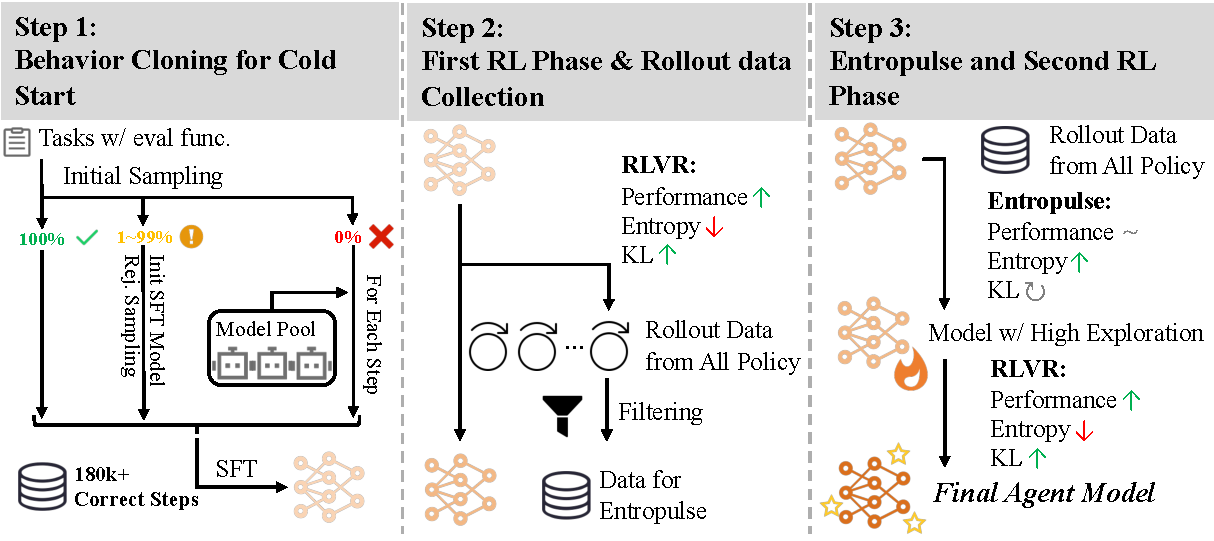
\includegraphics[width=0.95\textwidth]{images/training.pdf}
    \vspace{-1mm}
    \caption{\computerrl 概览，包含三个阶段：(1) 使用通用 LLM 收集的轨迹进行 BC 冷启动；(2) 使用可验证、基于规则的奖励进行步骤级 GRPO 强化学习；(3) \rlmethod，在 RL 与基于正确 rollout 的 SFT 之间交替，以恢复熵并维持学习。}
    \vspace{-3mm}
    \label{figs:main}
\end{figure}

我们系统地汇总并筛选所收集的交互数据，只保留成功轨迹（超过 \textbf{18 万个}正确步骤），并用它们对模型进行监督微调。
这一策略使模型获得稳健的桌面操作能力与基础推理能力，显著提升基础模型的性能。

\subsection{采用可验证奖励的强化学习}\label{sec:rlvr}

\textbf{步骤级组相对策略优化。}
我们将 GRPO 算法~\citep{shao2024deepseekmath}扩展到步骤级，使其更适合智能体 RL 训练。对于每个任务 $\tau$，策略 $\pi_{\theta}$ 与桌面环境交互，并采样 $G$ 条轨迹 $\mathcal{T}_1, \mathcal{T}_2, \ldots, \mathcal{T}_G$。
第 $i$ 条轨迹由 $L_i$ 个步骤级动作 $o_{i,1}, \ldots, o_{i,L_i}$ 组成。
来自同一任务的所有步骤被归为一组，并为每一步计算优势 $A_{i,j}$。
总损失按如下方式汇总所有步骤的优势：
\begingroup\small
\begin{align*}
\mathcal{J}_{StepGRPO}(\theta) = &\; \mathbb{E}_{\mathcal{T} \sim P(\mathcal{T}), \left\{\{o_{i,j}\}_{j=1}^{L_i}\right\}_{i=1}^{G} \sim \pi_{\theta_{old}}} \Bigg[\frac{1}{\sum_{i=1}^{G} L_i} \sum_{i=1}^{G} \sum_{j=1}^{L_i} \Bigg(\min \Bigg( \frac{\pi_{\theta}(o_{i,j}|q_{i,j})}{\pi_{\theta_{old}}(o_{i,j}|q_{i,j})} A_{i,j}, \\
    & \qquad \text{clip} \Big( \frac{\pi_{\theta}(o_{i,j}|q_{i,j})}{\pi_{\theta_{old}}(o_{i,j}|q_{i,j})}, 1 - \epsilon, 1 + \epsilon \Big) A_{i,j} \Bigg) - \beta \mathbb{D}_{KL}(\pi_{\theta} \| \pi_{ref}) \Bigg) \Bigg],
\end{align*}
\[
A_{i,j} = \frac{r_{i,j} - \text{mean}(\mathcal{R})}{\text{std}(\mathcal{R})}, \quad \mathcal{R} = \{ r_{u,v} \mid u=1,\dots,G, \, v=1,\dots,L_u \}
\]
\endgroup

\textbf{奖励设计。}
我们从构建的人工标注数据（见第~\ref{sec:bc-training}节）中选取一个子集用于 RL，并采用基于规则的验证函数，为每条轨迹提供可验证的训练信号。
对于成功解决任务的轨迹，每个格式正确且对解决任务有贡献的动作都获得奖励 1；失败轨迹或格式不正确的动作获得奖励 0。不同于通过贝尔曼方程传播逐步回报的传统方法，我们的方法将每一组提示—响应视为独立训练实例，并根据最终轨迹结果赋予奖励。通过将智能体行为与任务成功直接耦合，这种直接奖励分配方式提供了明确反馈，从而促进有效的策略优化。

\subsection{使用 \rlmethod 扩展 RL 训练}\label{sec:rewarm-rl}
在第~\ref{sec:rlvr}节的 RL 训练中，我们观察到，经过数百个训练步骤后模型性能便进入平台期，任务完成率停滞且熵持续下降。这种过早收敛促使我们研究如何延长有效训练并增强策略探索。
受 DAPO~\citep{yu2025dapo}启发，我们尝试提高裁剪阈值；这一做法减缓了熵的下降，却也显著降低了策略改进速度。

为解决这一问题，我们提出 \rlmethod。其动机来自我们的观察：SFT 与 RL 的目标在训练期间存在显著差异。随着 RL 优化过程中熵逐渐下降，在关键节点引入 SFT 可以增强探索与轨迹多样性，从而促进进一步的策略优化。
在初始 RL 训练期间，我们汇总并保留所有成功的 rollout 轨迹。按照惯例，这些轨迹使用一次后便会被丢弃；然而，它们来自不同训练步骤中的不同策略，是有价值且多样的行为数据。

我们处理该数据集时，会针对每个不同任务随机选择成功轨迹，构建新的 SFT 训练集。该训练集具有以下属性：
\begin{enumerate}[leftmargin=1.5em,itemsep=0pt,parsep=0.2em,topsep=0.0em,partopsep=0.0em]
    \item \textbf{高质量：}所有数据均由完整、高保真的轨迹组成。
    \item \textbf{多样性：}Rollout 来自不同训练步骤中的异构策略，因而包含多种问题求解策略。
    \item \textbf{计算高效：}该数据集利用已有交互数据，无需额外进行环境 rollout。
\end{enumerate}

在这一精选数据集上进行 SFT，会使策略行为发生显著变化。虽然评测任务性能保持稳定，但得到的策略相较原始策略具有更高的熵，表明其探索能力得到增强。
在这一增强的探索能力之上，我们开展第二轮 RL 训练，取得了显著的性能提升，并最终在计算机自动化任务中达到最先进水平。
训练细节见附录~\ref{apdx:training_details}。
